\chapter{Machine Learning Basics}
\section{What is Machine Learning}
\textit{A computer program is said to learn from experience E with respect to some class of tasks T and performance measure P, if its performance at tasks in T, as measured by P, improves with experience E.} Basically, Machine Learning is the field of study that gives computers the ability to learn without being explicitly programmed. In fact, we use Machine Learning when its impossible to \textbf{exactly formalise} the problem (and so to give an algorithmic solution) or when formulating a solution it's very complex and cannot be done manually.
\subsection{Main Learning Paradigms}
\begin{itemize}
    \item \textbf{Supervised Learning:}
    \begin{itemize}
        \item \textbf{Goal: }give the \textit{right answer} for each example in the data.
        \item Given a training set $\{(x^{(i)}, y^{(i)})\}$ we look for a function $h(\cdot)$ which is able to map in a predictive way $x^{(i)}$'s to $y^{(i)}$'s. It's called supervised learning because there is an expert that provides a \textit{supervision} assigning a label $y^{(i)}$ to each input $x^{(i)}$ 
        \item \textbf{Output: }Classification, regression.
        \item Use cases: Object recognition, Predicting pandemic, ... 
    \end{itemize}
    \begin{center}
        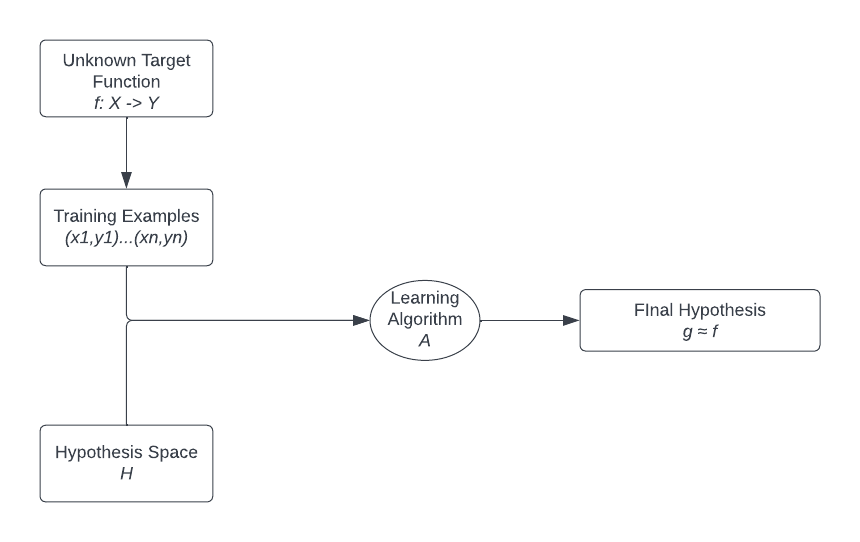
\includegraphics[scale=0.8]{images/Supervised Learning Diagram.png}
    \end{center}
    The \textit{Training examples} are generated according to the \textit{Target function $f$} (unknown). Once we have this set of pairs, we choose the \textit{hypothesis space}. The \textit{learning algorithm} (e.g a Neural Network) searches in the hypothesis space for a function $g$ that approximates the target function $f$.
    \item \textbf{Unsupervised Learning:}
    \begin{itemize}
        \item \textbf{Goal:} Find regularities / patterns on the data
        \item Given examples $\{x^{(i)}\}$, discover regularities on the whole input domain.
        \item There is no supervision.
        \item Use cases: Community detection in social media, user profiling, market analysis ...
    \end{itemize}    
    \item \textbf{Reinforcement Learning:}
    An \textbf{Agent} operates in an environment $e$, which in response to action $a$ (given by the agent) in the state $s$ returns the next state and a reward $r$ (which can be positive, negative or neutral).
    The goal of the Agent is to maximize a reward function.
    \begin{itemize}
        \item Use cases: Robotics, Games, ...
    \end{itemize}
    \begin{center}
        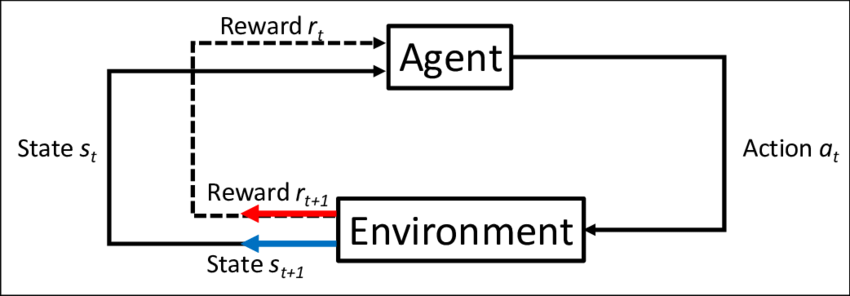
\includegraphics{images/Reinforcement learning.png}
    \end{center}
    \item \textbf{Other Learning Strategies:}
    \begin{itemize}
        \item Active Learning
        \item Online Learning, Incremental \& Continual Learning
        \item Weak Supervised Learning
        \item Self-supervised Learning
        \item Deep Learning and Representation Learning
        \item Federated Learning
    \end{itemize}
\end{itemize}

\subsection{Supervised Learning Keywords}

\begin{itemize}
\item \textbf{Input/Instance space x $\in X$:}
Representation of model's input (e.g. you can choose a Vector as a representation for your input). It contains all the possible inputs for a model. Suppose the model takes in a vector, $input = [x1, x2], x1,x2 \in [1,10]$, then we have $10^2$ possible inputs.
\item \textbf{Output space $y \in Y$:}
In supervised learning we want to perform a prediction based on the input. This prediction can be in the form of:
\begin{itemize}
    \item Binary Classification $y \equiv \{-1, +1\}$
    \item Multi-Class Classification $y \equiv \{1,...,m\}$
    \item Regression $y \equiv \mathbb{R}$
\end{itemize}
\item \textbf{Oracle/Nature:}
It determines how examples are generated. We can have two cases of Oracle
\begin{itemize}
    \item Target function $f: X \rightarrow Y$ It's deterministic and given an object of the input space returns an object of the output space. This function is ideal and \textbf{unknown}.
    \item Probability distribution $P(\textbf{x}), P(y\mid\textbf{x})$ The \textit{selection} of $y$ occurs from a probability distribution. This distribution is still unknown
\end{itemize}
\item \textbf{Training set:}
Set of pairs $\{(\textbf{x}_{1}, y_{1}), ..., (\textbf{x}_{n}, y_{n}) \}$ where each pair is composed by an instance of the input space and it's corresponding label.
\begin{center}
    \begin{tabular}{c|c}
     \textbf{x} & y\\
     000&0  \\
     001&1 \\
     010&1 \\
     .&. \\
     .&. \\
     .&.\\
    \end{tabular}
\end{center}
Data are typically:
\begin{itemize}
    \item Independent: Given two pairs $A,B$ $P(A \mid B) = P(A)$. The choice of one pair is independent from the choice of other pairs.
    
    \item Identically distributed: All pairs are generated by the same probability distribution (the Oracle) $P(\textbf{x},y) = P(\textbf{x})P(y\mid \textbf{x})$. \textit{Concept drift} is when data aren't identically distributed
\end{itemize}
\item \textbf{Hypothesis space:}
A \textbf{predefined} set of hypothesis/functions $H \equiv \{h\mid h:X \rightarrow Y\}$

\item \textbf{Empirical error/risk:}
Discrepancy between the target function $f$ and my approximation of that function $g \in H$ (chosen from the hypothesis space) \textbf{on training data}. For example, in a binary classification problem we can compute empirical error as follows:
\begin{center}
    \[\frac{1}{n}\sum_{i=1}^{n} [\![y_{i}\neq g(\textbf{x}_{i})]\!]\]
\end{center}
where $[\![\cdot]\!]$ is a function that is 1 if $\cdot$ is true and 0 otherwise.

\item \textbf{Ideal error:}
The \textbf{expected} error on given hypothesis $g$ and pairs $(\textbf{x},y)$. This can only be estimated. One way to estimate this quantity is testing the model over new examples that are not in the training set (test set) 

\item \textbf{Inductive bias:}
Since the hypothesis space can't contain all possible functions, we must make assumptions about the type of the unknown target function. The inductive bias consists of:
\begin{itemize}
    \item The hypothesis space: how $H$ is defined
    \item The learning algorithm: how $H$ is explored
\end{itemize}
\textbf{Examples of Inductive bias:}
\begin{itemize}
    \item \textbf{Hyperplanes in} $\mathbb{R}^{2}$: We chose as input space points in the plane $X = \{y\mid y \in \mathbb{R}^{2}\}$, and as hypothesis space the dichotomies induced by hyperplanes in $\mathbb{R}^{2}$, that is, $H = \{f_{w,b}(y) = sign(\textbf{w} \cdot y + b), \textbf{w} \in \mathbb{R}^{2}, b \in\mathbb{R}\}$.
    \begin{center}
        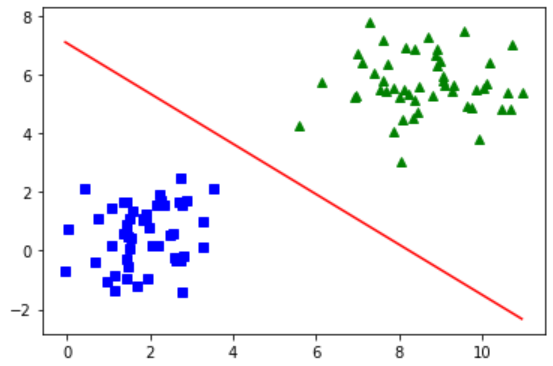
\includegraphics{Hyperplanes in R^2}
    \end{center}

    In this case the assumption is that examples are linearly separable
    
    \item \textbf{Polynomial functions}:
    Given a training set $S = \{(x_{1},y_{1}),...,(x_{n}, y_{n})\}, x\in \mathbb{R}, y\in \mathbb{R}$, the hypothesis space is the one containing functions of type: $h_{w}(x) = w_{0} + w_{1}x + w_{2}x^{2} + ... + w_{p}x^{p}, p\in \mathbb{N}$. The assumption is on the degree $p$ of the polynomial function.
    \begin{center}
        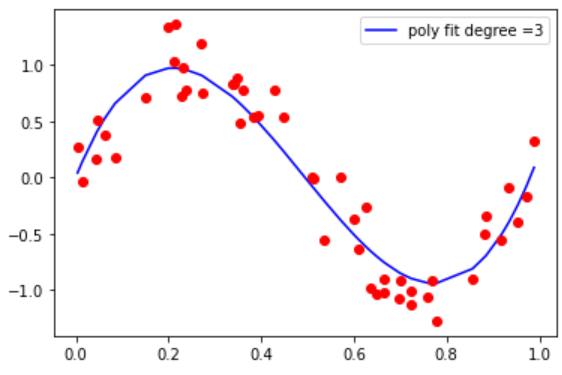
\includegraphics{images/Poly reg.png}
    \end{center}
\end{itemize}
\textbf{Bias-Variance Tradeoff:}
The learning goal is to find the best tradeoff between bias and variance.
\begin{itemize}
    \item The \textbf{bias} error is produced by weak assumptions in the learning algorithm. High bias can cause an algorithm to miss relevant relations between features and target outputs (\textbf{underfitting}).
    \item The \textbf{variance} is an error produced by an over-sensitivity to small fluctuations in the training set. High variance can cause an algorithm to model the random noise in the training data, rather than the intended outputs (\textbf{overfitting}).
    \begin{center}
        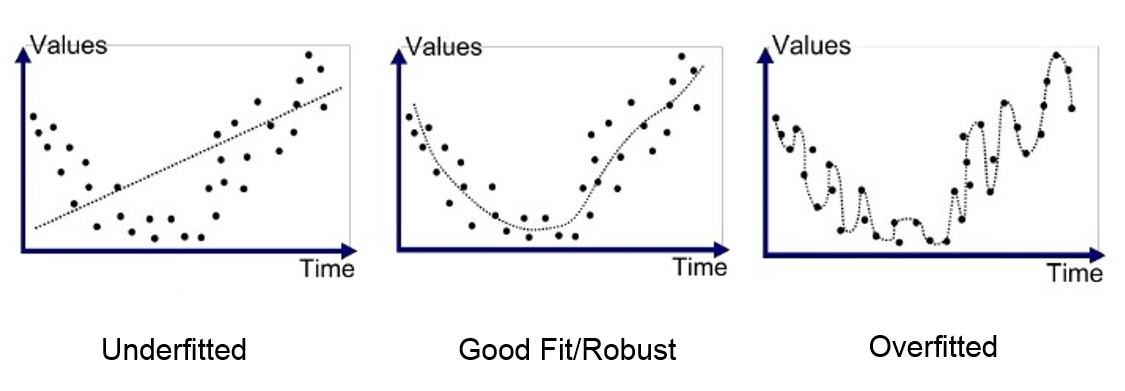
\includegraphics[scale = 0.35]{images/Overfitting vs Underfitting.png}
    \end{center}
\end{itemize}
\end{itemize}

